\subsection{To-do list}

\UC{Creare una lista}{UC2.1}

\begin{figure}[H]
	\centering
	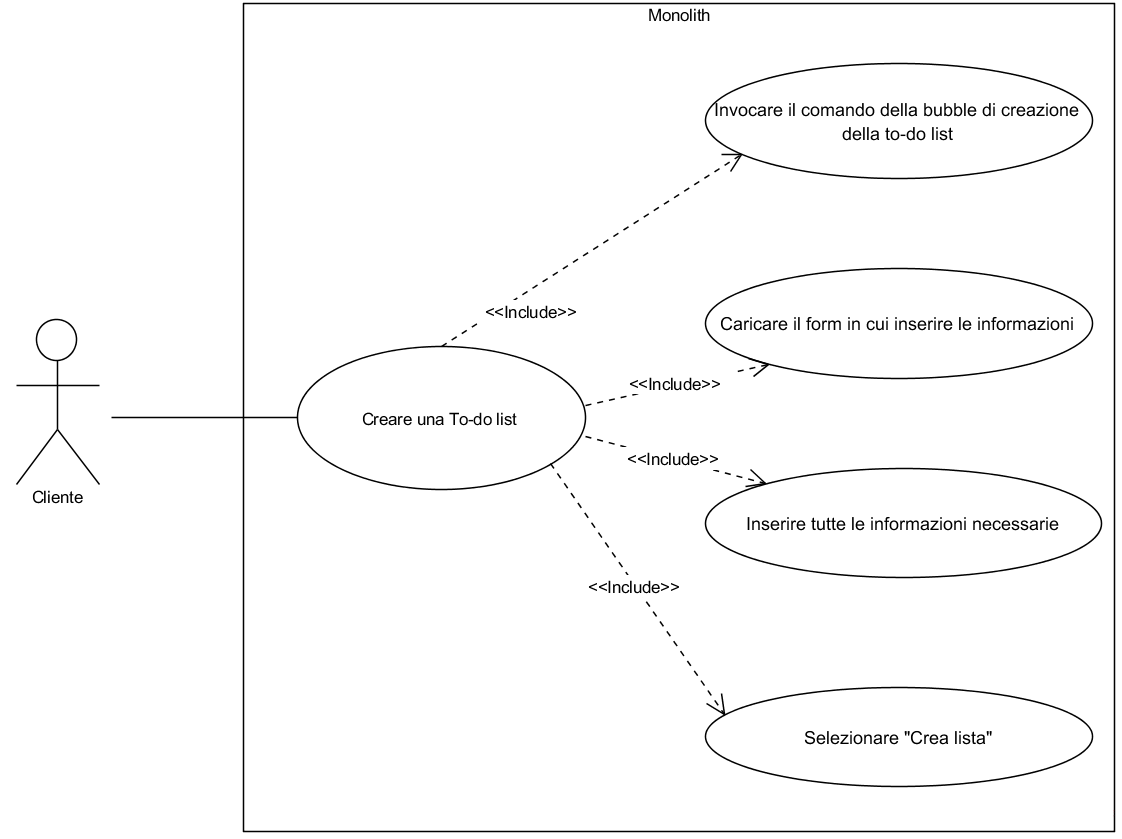
\includegraphics[width=15cm]{../../documenti/AnalisiDeiRequisiti/Diagrammi_img/uc2_1.png}
	\caption{\UCCaption{} Creare una lista}
\end{figure}

\begin{itemize}
	\item \textbf{Attori:}
	\\Utente di Rocket.Chat in possesso di \ProjectName{}.
	\item \textbf{Scopo e descrizione:} 
	\\Creare una lista di cose da fare.
	\item \textbf{Precondizioni:}
	\begin{itemize}
		\item Essere utenti di Rocket.Chat.
		\item Avere \ProjectName{} installato.
	\end{itemize}
	\item \textbf{Flusso principale degli eventi:}
	\begin{itemize}
		\item L'utente invoca il comando di creazione della bubble To-do list \ref{UC2.1.1}.
		\item L'utente carica il form in cui inserire le informazioni \ref{UC2.1.2}.
		\item L'utente inserisce tutte le informazioni necessarie \ref{UC2.1.3}.
		\item L'utente seleziona \virgolette{Crea lista} \ref{UC2.1.4}.
	\end{itemize}
	\item \textbf{Post-condizione:}
	\\Nella conversazione è presente una bubble To-do list con il titolo indicato.
\end{itemize}

\UCF{Invocare il comando della bubble di creazione della to-do list}{UC2.1.1}

\begin{itemize}
	\item \textbf{Attori:}
	\\Utente di Rocket.Chat in possesso di \ProjectName{}.
	\item \textbf{Scopo e descrizione:} 
	\\Creare una to-do list all'interno della chat.
	\item \textbf{Precondizioni:}
	\begin{itemize}
		\item Essere utenti di Rocket.Chat.
		\item Avere \ProjectName{} installato.
		\item Avere accesso alla bubble To-do list.
	\end{itemize}
	\item \textbf{Flusso principale degli eventi:}
	\\L'utilizzatore di \ProjectName{} utilizzando l'apposito comando inizia la creazione della bubble To-do list.
	\item \textbf{Post-condizione:}
	\\Viene istanziata la bubble.
\end{itemize}

\UCF{Caricare il form in cui inserire le informazioni}{UC2.1.2}

\begin{itemize}
	\item \textbf{Attori:}
	\\Utente di Rocket.Chat in possesso di \ProjectName{}.
	\item \textbf{Scopo e descrizione:} 
	\\Creare una to-do list all'interno della chat.
	\item \textbf{Precondizioni:}
	\begin{itemize}
		\item Essere utenti di Rocket.Chat.
		\item Avere \ProjectName{} installato.
		\item Aver invocato il comando di creazione della to-do list \ref{UC2.1.1}.
	\end{itemize}
	\item \textbf{Flusso principale degli eventi:}
	\\Viene caricato il form per l'inserimento delle informazioni.
	\item \textbf{Post-condizione:}
	\\Nella conversazione è presente una bubble To-do list con al suo interno un form per l'inserimento delle informazioni necessarie al completamento della creazione della to-do list.
\end{itemize}

\UCF{Inserire tutte le informazioni necessarie}{UC2.1.3}

\begin{itemize}
	\item \textbf{Attori:}
	\\Utente di Rocket.Chat in possesso di \ProjectName{}.
	\item \textbf{Scopo e descrizione:} 
	\\Specificare le informazioni necessarie alla creazione della lista.
	\item \textbf{Precondizioni:}
	\begin{itemize}
		\item Essere utenti di Rocket.Chat.
		\item Avere \ProjectName{} installato.
		\item Aver caricato il form di inserimento secondo \ref{UC2.1.2}.
	\end{itemize}
	\item \textbf{Flusso principale degli eventi:}
	\\L'utilizzatore della bubble inserisce i dati necessari nel form visualizzato al caso d'uso \ref{UC2.1.2}.
	\item \textbf{Post-condizione:}
	\\Nella memoria della bubble sono salvati i dati richiesti nel caso d'uso \ref{UC2.1.4}. 
\end{itemize}

\UCF{Selezionare \virgolette{Crea lista}}{UC2.1.4}

\begin{itemize}
	\item \textbf{Attori:}
	\\Utente di Rocket.Chat in possesso di \ProjectName{}.
	\item \textbf{Scopo e descrizione:} 
	\\Creazione di una lista di cose da fare.
	\item \textbf{Precondizioni:}
	\begin{itemize}
		\item Essere utenti di Rocket.Chat.
		\item Avere \ProjectName{} installato.
		\item Sono stati inseriti i dati come da \ref{UC2.1.3}.
	\end{itemize}
	\item \textbf{Flusso principale degli eventi:}
	\\Viene utilizzato l'apposito comando per la creazione effettiva della lista all'interno della bubble.
	\item \textbf{Post-condizione:}
	\\Nella conversazione è presente una bubble To-do list con il titolo indicato. 
\end{itemize}

\UC{Aggiungere elemento alla to-do list}{UC2.2}

\begin{figure}[H]
	\centering
	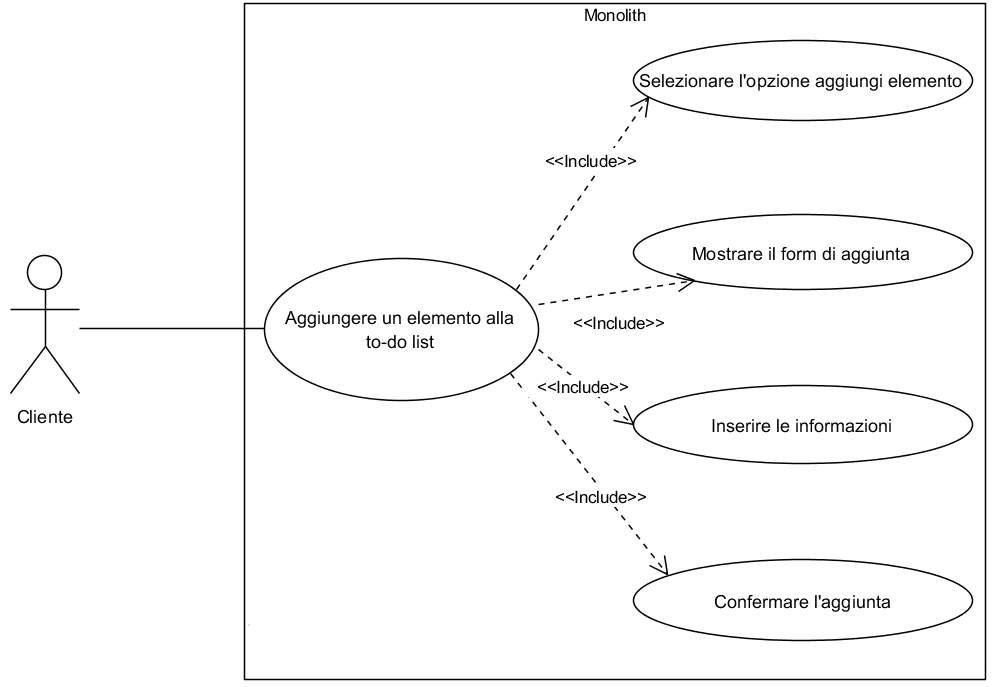
\includegraphics[width=15cm]{../../documenti/AnalisiDeiRequisiti/Diagrammi_img/uc2_2.png}
	\caption{\UCCaption{} Aggiungere elemento alla to-do list}
\end{figure}

\begin{itemize}
	\item \textbf{Attori:}
	\\Utente di Rocket.Chat in possesso di \ProjectName{}.
	\item \textbf{Scopo e descrizione:} 
	\\Un utente inserisce un nuovo elemento\footnote{Sono considerati elementi per la to-do list le voci testuali e/o con immagini.} alla to-do list.
	\item \textbf{Precondizioni:}
	\begin{itemize}
		\item Avere ricevuto una bubble To-do list.
		\item L'elemento non è già stato completato.
	\end{itemize}
	\item \textbf{Flusso principale degli eventi:}
	\begin{itemize}
		\item L'utente seleziona l'opzione aggiungi elemento \ref{UC2.2.1}.
		\item Mostrare il form di aggiunta \ref{UC2.2.2}.
		\item L'utente inserisce le informazioni \ref{UC2.2.3}.
		\item L'utente conferma l'aggiunta \ref{UC2.2.4}.
	\end{itemize}
	\item \textbf{Post-condizione:}
	\\La to-do list avrà il nuovo elemento aggiunto.
\end{itemize}

\UCF{Selezionare l'opzione aggiungi elemento}{UC2.2.1}

\begin{itemize}
	\item \textbf{Attori:}
	\\Utente di Rocket.Chat in possesso di \ProjectName{}.
	\item \textbf{Scopo e descrizione:} 
	\\L'utente seleziona l'opzione per inserire un nuovo elemento alla to-do list.
	\item \textbf{Precondizioni:}
	\begin{itemize}
		\item Avere ricevuto una bubble To-do list.
	\end{itemize}
	\item \textbf{Flusso principale degli eventi:}
	\\L'utilizzatore del metodo seleziona l'opzione apposita.
	\item \textbf{Post-condizione:}
	\\È possibile inserire il testo per il nuovo elemento. 
\end{itemize}

\UCF{Mostrare il form di aggiunta}{UC2.2.2}

\begin{itemize}
	\item \textbf{Attori:}
	\\Utente di Rocket.Chat in possesso di \ProjectName{}.
	\item \textbf{Scopo e descrizione:} 
	\\Visualizzazione del form di aggiunta delle informazioni relative al nuovo elemento della to-do list.
	\item \textbf{Precondizioni:}
	\begin{itemize}
		\item Avere ricevuto una bubble To-do list.
		\item Avere selezionato l'opzione aggiungi elemento come da \ref{UC2.2.1}.
	\end{itemize}
	\item \textbf{Flusso principale degli eventi:}
	\\L'utilizzatore del metodo scrive il testo da inserire nel nuovo elemento e lo aggiunge alla to-do list.
	\item \textbf{Post-condizione:}
	\\Il nuovo elemento è aggiunto alla bubble To-do list.
\end{itemize}

\UCF{Inserire le informazioni}{UC2.2.3}

\begin{itemize}
	\item \textbf{Attori:}
	\\Utente di Rocket.Chat in possesso di \ProjectName{}.
	\item \textbf{Scopo e descrizione:} 
	\\L'utente inserisce le informazioni necessarie ad aggiungere un elemento alla to-do list.
	\item \textbf{Precondizioni:}
	\begin{itemize}
		\item Avere ricevuto una bubble To-do list.
		\item Aver caricato il form di inserimento secondo \ref{UC2.2.2}.
	\end{itemize}
	\item \textbf{Flusso principale degli eventi:}
	\\L'utilizzatore del metodo completa il form di inserimento di un nuovo elemento in tutte le sue parti.
	\item \textbf{Post-condizione:}
	\\La to-do list ha tutte le informazioni necessarie per aggiungere il nuovo elemento.
\end{itemize}

\UCF{Confermare l'aggiunta}{UC2.2.4}

\begin{itemize}
	\item \textbf{Attori:}
	\\Utente di Rocket.Chat in possesso di \ProjectName{}.
	\item \textbf{Scopo e descrizione:} 
	\\Un utente conferma l'inserimento del nuovo elemento alla to-do list.
	\item \textbf{Precondizioni:}
	\begin{itemize}
		\item Avere ricevuto una bubble To-do list.
		\item Aver inserito le informazioni per il nuovo elemento secondo \ref{UC2.2.3}.
	\end{itemize}
	\item \textbf{Flusso principale degli eventi:}
	\\L'utilizzatore del metodo conferma l'aggiunta alla to-do list.
	\item \textbf{Post-condizione:}
	\\L'elemento è stato aggiunto alla to-do list.
\end{itemize}

\UC{Indicare come completati gli elementi della to-do list}{UC2.3}

\begin{figure}[H]
	\centering
	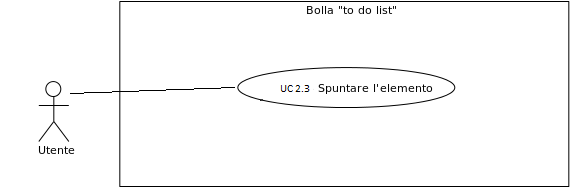
\includegraphics[width=15cm]{../../documenti/AnalisiDeiRequisiti/Diagrammi_img/uc2_3.png}
	\caption{\UCCaption{} Indicare come completati gli elementi della to-do list}
\end{figure}

\begin{itemize}
	\item \textbf{Attori:}
	\\Utente di Rocket.Chat in possesso di \ProjectName{} che abbia ricevuto come messaggio una bubble To-do list.
	\item \textbf{Scopo e descrizione:} 
	\\L'utente con questo metodo può indicare come completato uno degli elementi della lista.
	\item \textbf{Precondizioni:}
	\begin{itemize}
		\item Avere ricevuto una bubble To-do list.
		\item L'elemento non è già stato completato.
	\end{itemize}
	\item \textbf{Flusso principale degli eventi:}
	\\L'utilizzatore del metodo seleziona un elemento della to-do list e lo indica come completato. 
	\item \textbf{Post-condizione:}
	\\L'elemento della to-do list viene aggiornato come completato.
\end{itemize}

\UC{Possibilità di mettere un reminder come notifica statica}{UC2.4}

\begin{figure}[H]
	\centering
	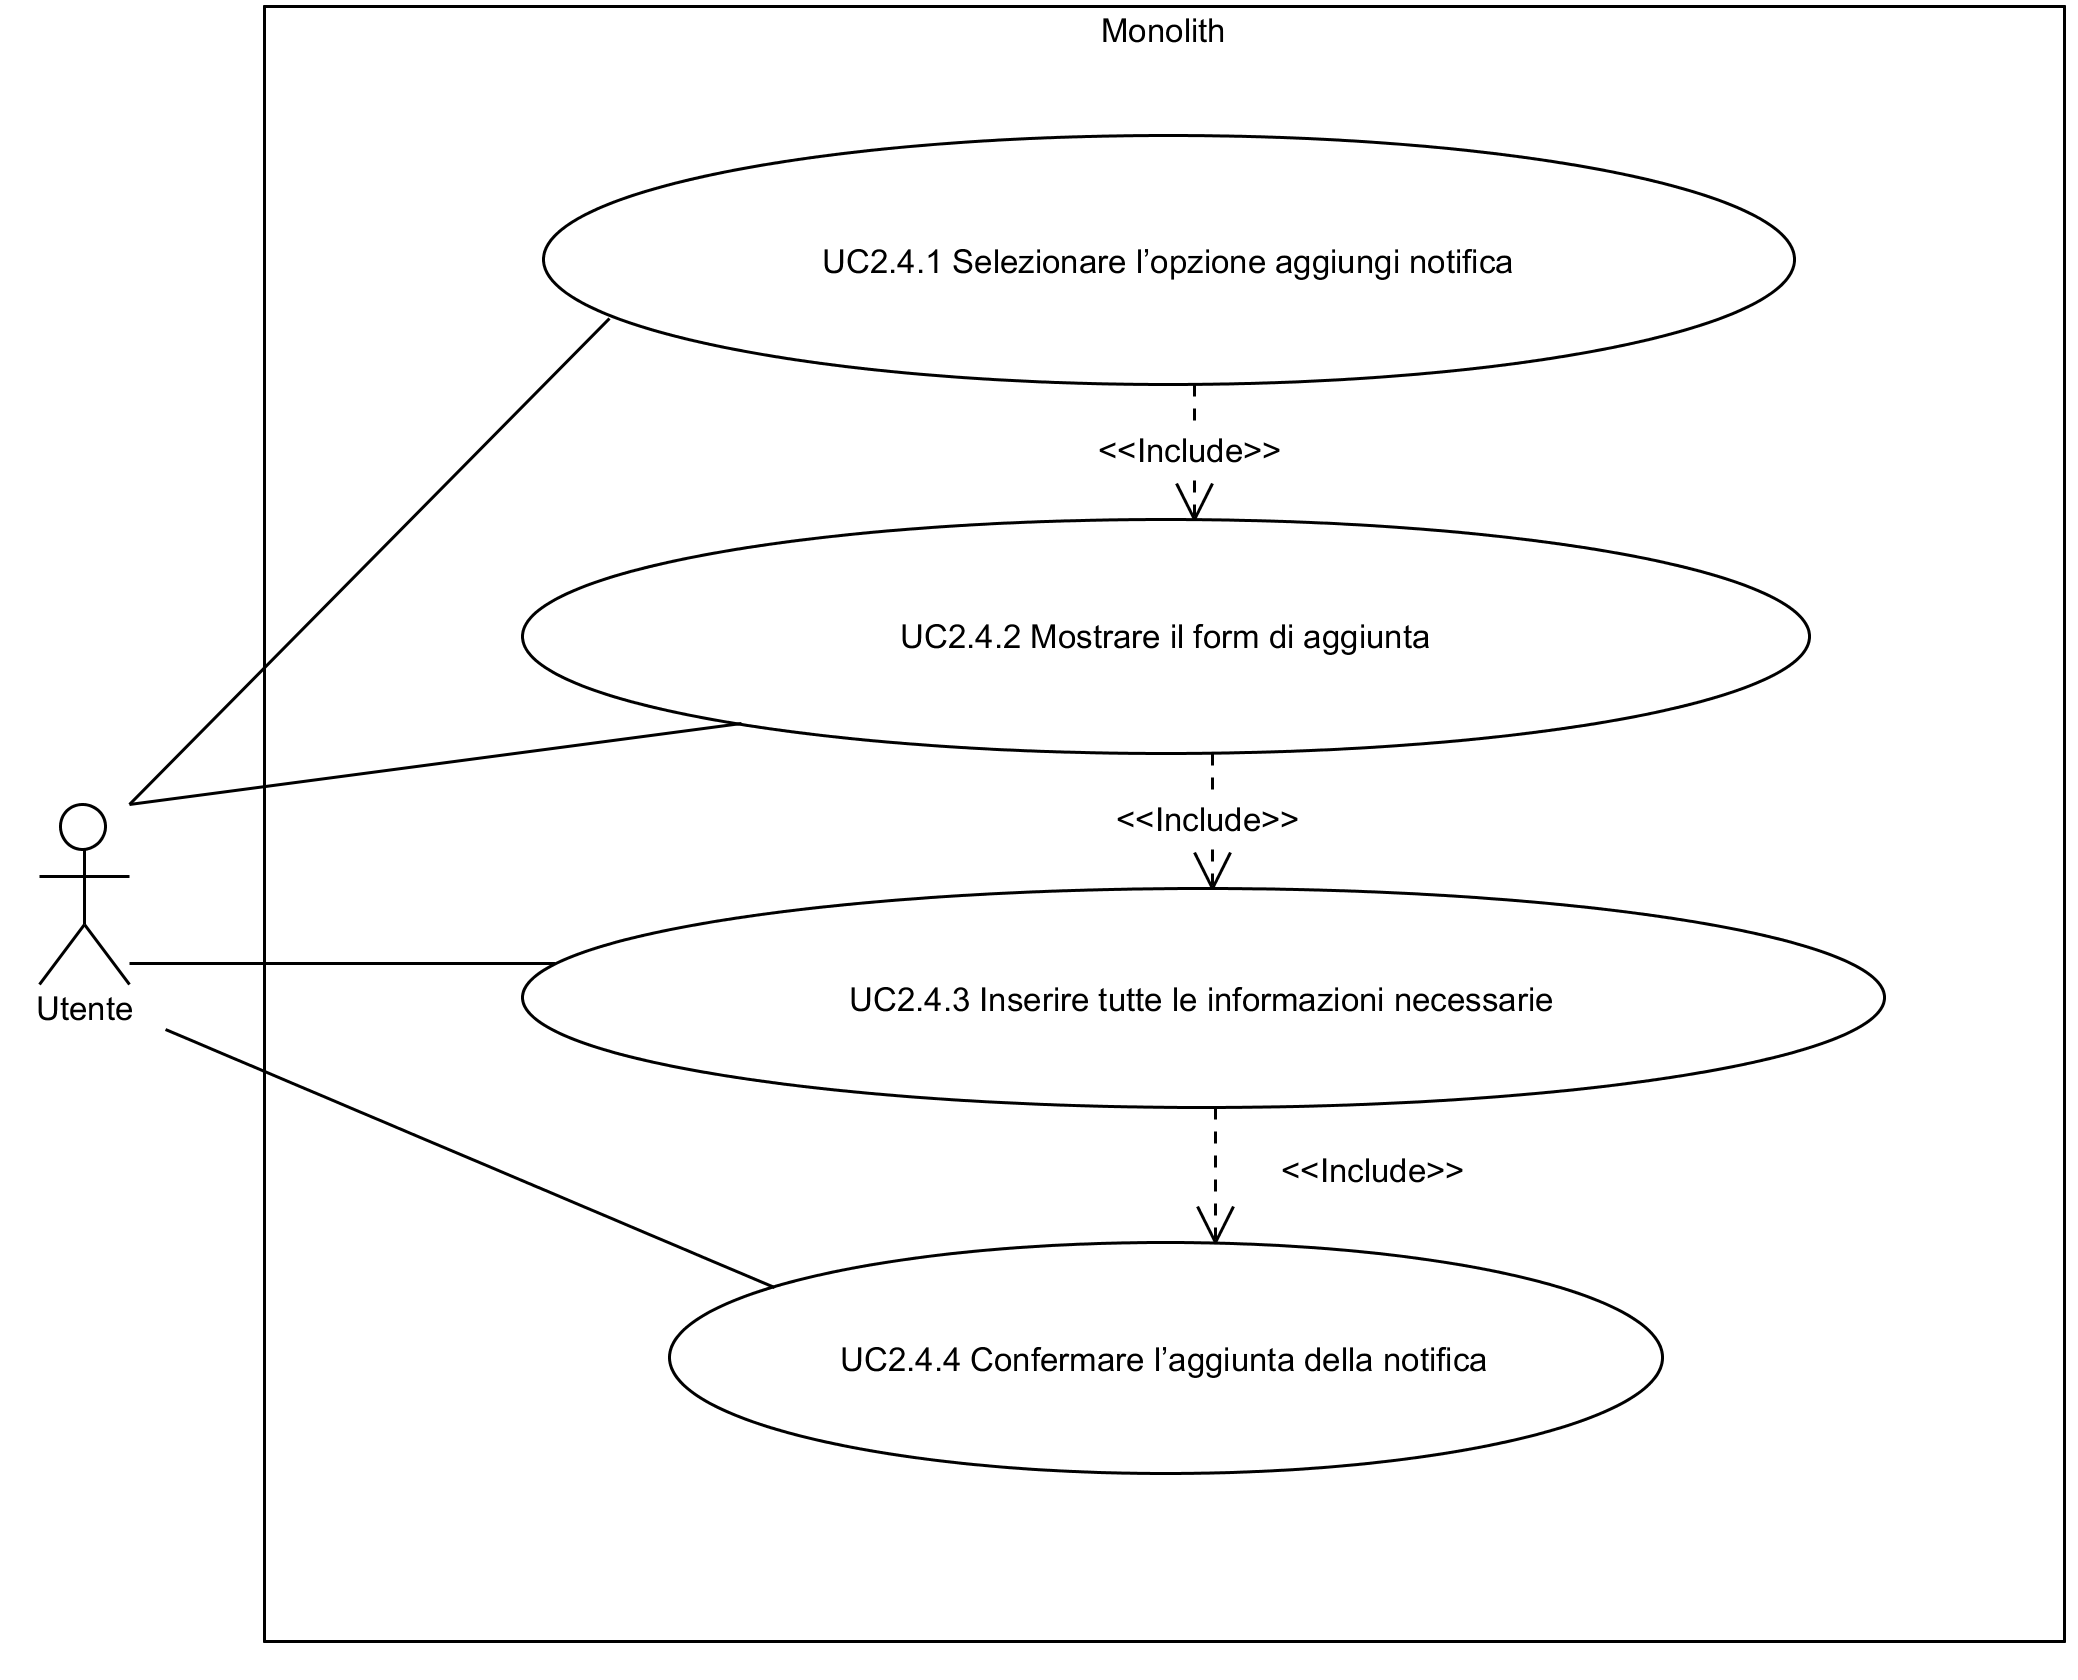
\includegraphics[width=15cm]{../../documenti/AnalisiDeiRequisiti/Diagrammi_img/uc2_4.png}
	\caption{\UCCaption{} Possibilità di mettere un reminder come notifica statica}
\end{figure}

\begin{itemize}
	\item \textbf{Attori:}
	\\Utente di Rocket.Chat in possesso di \ProjectName{} che ha creato la to-do list.
	\item \textbf{Scopo e descrizione:} 
	\\Il creatore della lista imposta una notifica statica da visualizzare ai membri del canale ad un orario specificato.
	\item \textbf{Precondizioni:}
	\begin{itemize}
		\item Avere ricevuto una bubble To-do list.
	\end{itemize}
	\item \textbf{Flusso principale degli eventi:}
	\begin{itemize}
		\item L'utente seleziona l'opzione aggiungi notifica \ref{UC2.4.1}.
		\item Mostrare il form di aggiunta \ref{UC2.4.2}.
		\item L'utente inserisce tutte le informazioni necessarie \ref{UC2.4.3}.
		\item L'utente conferma l'aggiunta della notifica \ref{UC2.4.4}.
	\end{itemize}
	\item \textbf{Post-condizione:}
	\\I partecipanti al gruppo nel quale è presente la bubble verranno notificati della lista all'ora specificata.
\end{itemize}

\UCF{Selezionare l'opzione aggiungi notifica}{UC2.4.1}

\begin{itemize}
	\item \textbf{Attori:}
	\\Utente di Rocket.Chat in possesso di \ProjectName{}.
	\item \textbf{Scopo e descrizione:} 
	\\Il creatore della lista seleziona l'opzione \virgolette{aggiungi notifica} per la to-do list che ha creato.
	\item \textbf{Precondizioni:}
	\begin{itemize}
		\item Avere creato una bubble To-do list.
	\end{itemize}
	\item \textbf{Flusso principale degli eventi:}
	\\L'utilizzatore del metodo seleziona l'opzione \virgolette{aggiungi notifica} sulla bubble.
	\item \textbf{Post-condizione:}
	\\L'utente ha selezionato l'opzione di aggiungere una notifica alla to-do list che ha creato.
\end{itemize}

\UCF{Mostrare il form di aggiunta}{UC2.4.2}

\begin{itemize}
	\item \textbf{Attori:}
	\\Utente di Rocket.Chat in possesso di \ProjectName{}.
	\item \textbf{Scopo e descrizione:} 
	\\Questa funzionalità permette alla bubble di caricare il form necessario ad inserire i dati per aggiungere una notifica alla bubble.
	\item \textbf{Precondizioni:}
	\begin{itemize}
		\item Avere ricevuto una bubble To-do list.
		\item Essere entrati nell'opzione \virgolette{aggiungi modifica} della propria bubble secondo \ref{UC2.4.1}.
	\end{itemize}
	\item \textbf{Flusso principale degli eventi:}
	\\La bubble To-do list carica il form di inserimento dati per le notifiche.
	\item \textbf{Post-condizione:}
	\\La bubble ha caricato il form ed è pronta a ricevere in input le informazioni sulla notifica.
\end{itemize}

\UCF{Inserire tutte le informazioni necessarie}{UC2.4.3}

\begin{itemize}
	\item \textbf{Attori:}
	\\Utente di Rocket.Chat in possesso di monolith.
	\item \textbf{Scopo e descrizione:} 
	\\Il creatore della lista completa il form di aggiunta notifica.
	\item \textbf{Precondizioni:}
	\begin{itemize}
		\item Avere ricevuto una bubble di to-do list.
		\item La bubble ha caricato il form di inserimento dati secondo lo \ref{UC2.4.2}.
	\end{itemize}
	\item \textbf{Flusso principale degli eventi:}
	\\L'utilizzatore del metodo inserirà tutte le informazioni necessarie a completare il form di aggiunta di una notifica.
	\item \textbf{Post-condizione:}
	\\La bubble possiede tutte le informazioni necessarie ad aggiungere una notifica alla to-do list.
\end{itemize}

\UCF{Confermare l'aggiunta della notifica}{UC2.4.4}

\begin{itemize}
	\item \textbf{Attori:}
	\\Utente di Rocket.Chat in possesso di \ProjectName{}.
	\item \textbf{Scopo e descrizione:} 
	\\Il creatore della lista conferma l'aggiunta della notifica.
	\item \textbf{Precondizioni:}
	\begin{itemize}
		\item Avere ricevuto una bubble To-do list.
		\item Aver completato il form di aggiunta di una notifica secondo lo \ref{UC2.4.3}.
	\end{itemize}
	\item \textbf{Flusso principale degli eventi:}
	\\L'utilizzatore del metodo seleziona l'opzione \virgolette{conferma aggiunta} e la bubble aggiunge la notifica alla lista.
	\item \textbf{Post-condizione:}
	\\La bubble ha aggiunto la notifica alla to-do list.
\end{itemize}

